% =============================================================================
% Material suplementar da versao RSBMT.
%
% Recebe as 9 ilustracoes que nao couberam no limite de 5 do texto principal.
% Usa exatamente os mesmos arquivos gerados por build_paper_assets.py, entao
% nenhum numero aqui e independente do manuscrito: sao a mesma fonte.
%
% A numeracao vira S1, S2, ... via \thetable e \thefigure.
%
% Compilar:  tectonic -X compile supplementary.tex --outdir ../build
% =============================================================================
\documentclass[11pt]{article}

\usepackage[margin=1in]{geometry}
\usepackage[T1]{fontenc}
\usepackage[utf8]{inputenc}
\usepackage{lmodern}
\usepackage{amsmath}
\usepackage{booktabs}
\usepackage{multirow}
\usepackage{graphicx}
\usepackage{xurl}
\usepackage{caption}

\captionsetup{font=small,labelfont=bf}
\graphicspath{{figures/}}

% numeracao suplementar
\renewcommand{\thetable}{S\arabic{table}}
\renewcommand{\thefigure}{S\arabic{figure}}
\renewcommand{\thesection}{S\arabic{section}}

\title{Supplementary material\\[4pt]
\large Zero-Shot Foundation Models Versus Purpose-Trained Models for Dengue
Forecasting in Eight Brazilian State Capitals (2010 to 2024)}

\author{Fabiano Barcellos-Filho \and Jos\'e Trajano \and Wilson Falco}
\date{}

\begin{document}

\maketitle

\noindent Every table and figure below is generated from the same analysis output as the
main text, by \texttt{scripts/build\_paper\_assets.py} in the project repository
(\url{https://github.com/fabianofilho/dengue-time-series}). No value here is computed
independently of the main manuscript.

\tableofcontents

% =============================================================================
\section{Burden and volatility of the eight series}

Table~\ref{tab:descriptive} gives the descriptive statistics summarised in the main text,
and Figure~\ref{fig:series} shows the eight series. Ranking by population-standardised
incidence rather than by absolute count moves S\~ao Paulo from first to fourth and places
Belo Horizonte first, which is the reordering reported in the Results.

% gerado por scripts/build_paper_assets.py -- nao editar a mao
\begin{table}[htbp]
\centering
\footnotesize
\setlength{\tabcolsep}{4pt}
\caption{Notified dengue burden in eight Brazilian state capitals, January 2010 to
December 2024: monthly case counts and population-standardised incidence.}
\label{tab:descriptive}
\begin{tabular}{llrrrrrrrr}
\toprule
 & & Pop. 2022 & \multicolumn{4}{c}{Monthly cases}
 & \multicolumn{3}{c}{Incidence per 100{,}000} \\
\cmidrule(lr){4-7} \cmidrule(lr){8-10}
City & Region & (millions) & Total & Median & Max & CV (\%)
 & Annual & Median & Max \\
\midrule
Belo Horizonte (MG) & Southeast & 2.32 & 1,081,180 & 948 & 113,951 & 262 & 3,124 & 41 & 4,938 \\
Brasilia (DF) & Central-West & 2.82 & 720,807 & 1,146 & 102,593 & 283 & 1,740 & 43 & 3,597 \\
Fortaleza (CE) & Northeast & 2.43 & 381,475 & 962 & 21,568 & 142 & 1,054 & 39 & 881 \\
Sao Paulo (SP) & Southeast & 11.45 & 1,702,694 & 1,192 & 342,838 & 432 & 1,002 & 10 & 2,986 \\
Recife (PE) & Northeast & 1.49 & 184,961 & 488 & 7,667 & 132 & 824 & 32 & 506 \\
Rio de Janeiro (RJ) & Southeast & 6.21 & 637,074 & 658 & 55,481 & 241 & 685 & 10 & 880 \\
Manaus (AM) & North & 2.06 & 132,030 & 274 & 19,556 & 285 & 472 & 14 & 1,078 \\
Salvador (BA) & Northeast & 2.42 & 116,190 & 344 & 4,088 & 106 & 312 & 13 & 171 \\
\bottomrule
\end{tabular}

\vspace{0.5em}
\begin{minipage}{\textwidth}
\footnotesize
Each city contributed 180 monthly observations. CV: coefficient of variation of the
monthly case count (standard deviation divided by the mean, as a percentage). Incidence
columns are notified cases per 100{,}000 inhabitants; Annual is the mean monthly
incidence multiplied by twelve, Median and Max are monthly values. Rows are sorted by
mean annual incidence, which reorders the table relative to absolute counts. Population
denominators are interpolated monthly from an annual series anchored on the 2010 and 2022
Censuses (see Methods). Case source: InfoDengue (Fiocruz/FGV); population source: IBGE.
\end{minipage}
\end{table}


\begin{figure}[htbp]
\centering
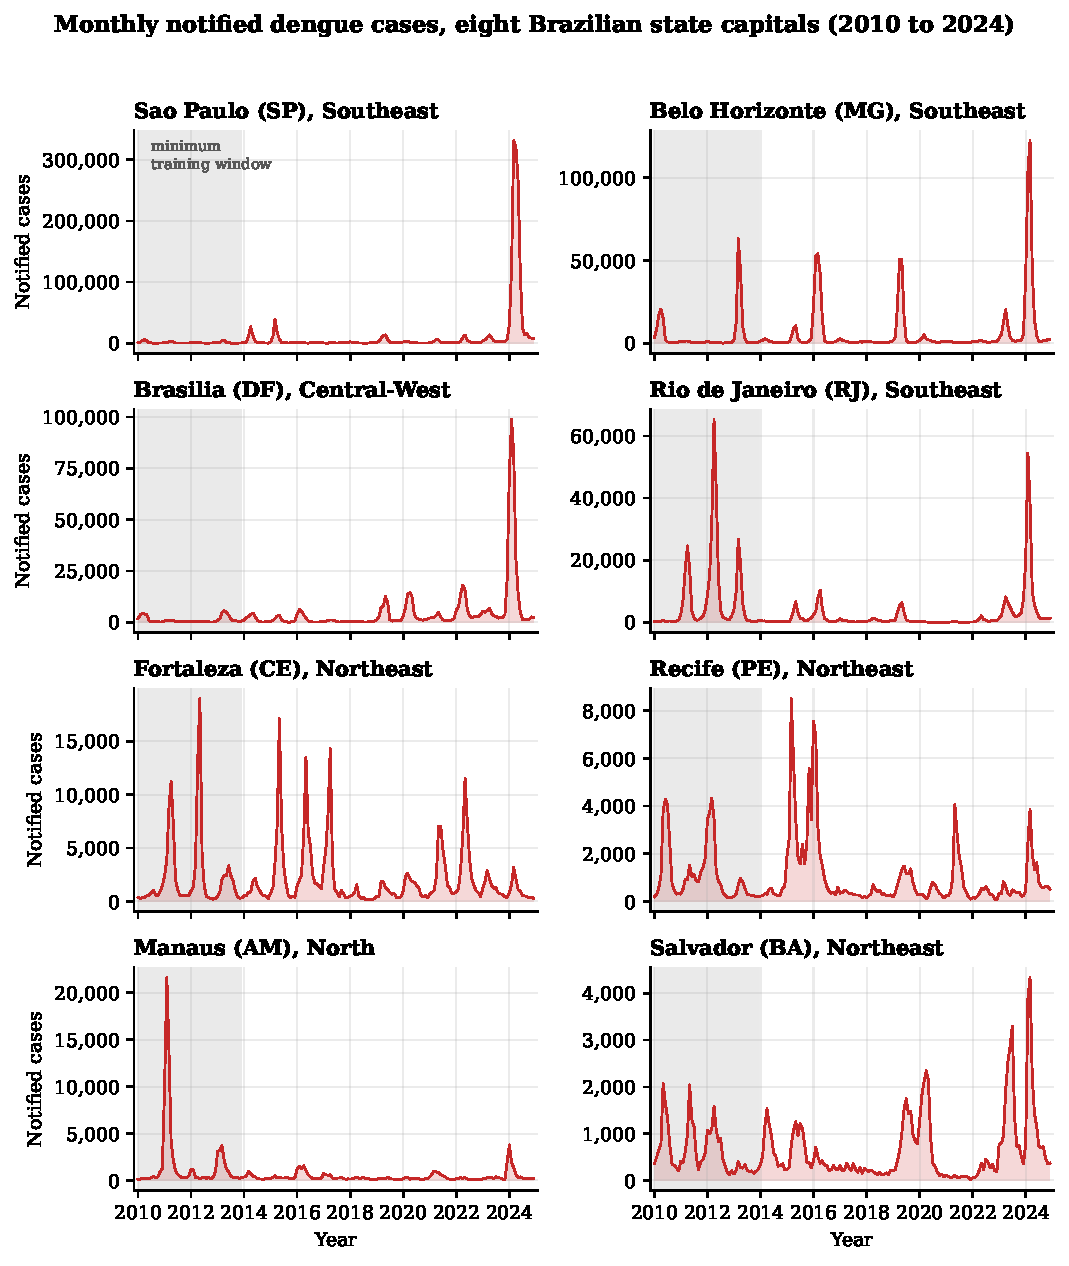
\includegraphics[width=\textwidth]{fig1_series.pdf}
\caption{Monthly notified dengue cases in eight Brazilian state capitals, February 2010 to
November 2024. Panels are ordered by cumulative case count and each has its own vertical
scale. The shaded band marks the 48-month minimum training window, before which no
forecast is evaluated. The 2024 epidemic is visible in all eight series.}
\label{fig:series}
\end{figure}

% =============================================================================
\section{Accuracy on the case-count scale}

The main text reports sMAPE, the pre-specified primary metric. Table~\ref{tab:mae-rmse}
gives mean absolute error and root mean squared error on the original scale, which are not
comparable across cities but show how much of the total error sits in a few months: where
RMSE greatly exceeds MAE, the error is concentrated at epidemic peaks. In S\~ao Paulo the
best MAE is 8{,}759 cases against an RMSE above 41{,}000 for every model.

% gerado por scripts/build_paper_assets.py -- nao editar a mao
\begin{table}[htbp]
\centering
\small
\setlength{\tabcolsep}{4pt}
\caption{Forecasting accuracy by model and city: mean absolute error (MAE) and root
mean squared error (RMSE), in notified cases per month.}
\label{tab:mae-rmse}
\begin{tabular}{llccccccc}
\toprule
City & Metric & TimesFM & CatBoost & XGBoost & Random Forest & SARIMAX & Ridge & LightGBM \\
\midrule
\multirow{2}{*}{Sao Paulo} & MAE & \textbf{8,759} & 9,142 & 10,074 & 9,659 & 76,493 & 11,300 & 10,283 \\
 & RMSE & 41,532 & 41,327 & 41,603 & 41,331 & 1,314,044 & 43,506 & \textbf{40,821} \\[2pt]
\multirow{2}{*}{Rio de Janeiro} & MAE & \textbf{1,899} & 4,487 & 8,357 & 7,368 & 2,481 & 4,920 & 5,507 \\
 & RMSE & \textbf{5,801} & 8,039 & 17,102 & 13,349 & 6,081 & 8,427 & 8,071 \\[2pt]
\multirow{2}{*}{Belo Horizonte} & MAE & \textbf{6,177} & 7,997 & 8,715 & 8,860 & 11,198 & 8,060 & 14,877 \\
 & RMSE & 16,840 & 17,631 & 20,454 & 18,749 & 21,838 & \textbf{16,684} & 21,097 \\[2pt]
\multirow{2}{*}{Brasilia} & MAE & 3,686 & \textbf{3,668} & 4,142 & 4,049 & 4,250 & 4,118 & 4,395 \\
 & RMSE & 12,444 & 11,989 & 12,456 & 12,155 & 12,032 & 12,315 & \textbf{11,678} \\[2pt]
\multirow{2}{*}{Fortaleza} & MAE & \textbf{1,417} & 1,960 & 3,291 & 3,386 & 1,856 & 1,935 & 3,053 \\
 & RMSE & \textbf{2,602} & 3,032 & 5,276 & 4,568 & 3,102 & 2,882 & 3,971 \\[2pt]
\multirow{2}{*}{Recife} & MAE & \textbf{755} & 1,159 & 1,160 & 1,173 & 1,345 & 1,159 & 1,700 \\
 & RMSE & \textbf{1,428} & 1,824 & 1,942 & 1,866 & 2,327 & 1,994 & 2,218 \\[2pt]
\multirow{2}{*}{Manaus} & MAE & \textbf{274} & 343 & 359 & 305 & 352 & 274 & 429 \\
 & RMSE & 556 & 578 & 634 & 531 & 618 & \textbf{529} & 641 \\[2pt]
\multirow{2}{*}{Salvador} & MAE & \textbf{416} & 472 & 517 & 502 & 595 & 518 & 567 \\
 & RMSE & \textbf{687} & 726 & 781 & 742 & 917 & 758 & 765 \\[2pt]
\bottomrule
\end{tabular}

\vspace{0.5em}
\begin{minipage}{\textwidth}
\footnotesize
Bold indicates the best value in each row. MAE and RMSE are reported on the original
case-count scale and are therefore not comparable across cities. RMSE penalises large
errors more heavily than MAE; the gap between the two within a city reflects how much
of the total error is concentrated in a small number of epidemic peaks.
\end{minipage}
\end{table}


\begin{figure}[htbp]
\centering
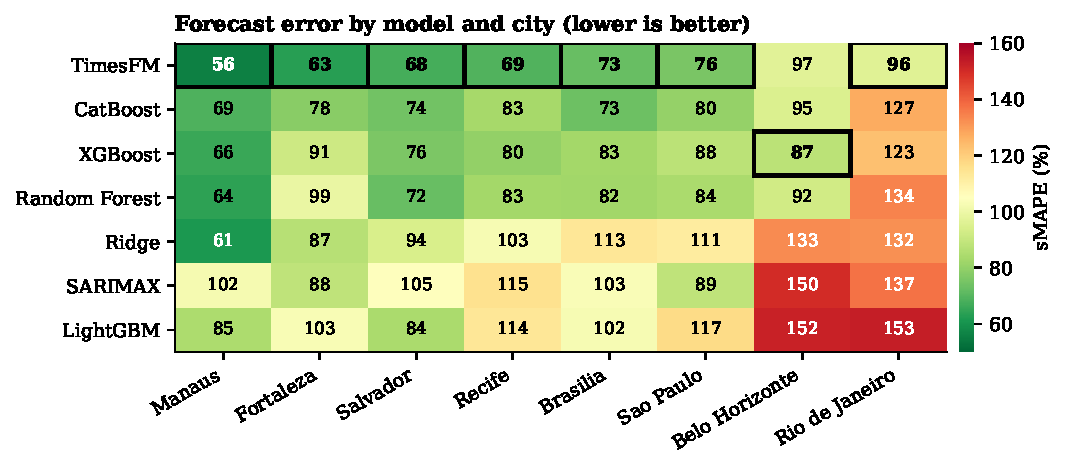
\includegraphics[width=\textwidth]{fig2_heatmap.pdf}
\caption{sMAPE by model and city. Cities are ordered by the lowest error achieved by any
model and models by mean sMAPE across cities. The outlined cell in each column is the best
model for that city. TimesFM holds the best cell in seven of eight columns; Belo Horizonte
is the exception.}
\label{fig:heatmap}
\end{figure}

% =============================================================================
\section{Which model each metric selects}

Table~\ref{tab:metric-disagreement} lists the winner per city under each of the three
accuracy metrics. The three agree in four of the eight cities. In Belo Horizonte and
Bras\'ilia each metric names a different model, which is the result summarised in the main
text.

% gerado por scripts/build_paper_assets.py -- nao editar a mao
\begin{table}[htbp]
\centering
\small
\caption{Best-performing model per city under each accuracy metric, showing where the
choice of metric changes the winner.}
\label{tab:metric-disagreement}
\begin{tabular}{llllc}
\toprule
City & Best by sMAPE & Best by MAE & Best by RMSE & All three agree \\
\midrule
Sao Paulo & TimesFM & TimesFM & LightGBM & No \\
Rio de Janeiro & TimesFM & TimesFM & TimesFM & Yes \\
Belo Horizonte & XGBoost & TimesFM & Ridge & No \\
Brasilia & TimesFM & TimesFM & SARIMAX & No \\
Fortaleza & TimesFM & TimesFM & TimesFM & Yes \\
Recife & TimesFM & TimesFM & TimesFM & Yes \\
Manaus & TimesFM & TimesFM & Random Forest & No \\
Salvador & TimesFM & TimesFM & TimesFM & Yes \\
\bottomrule
\end{tabular}

\vspace{0.5em}
\begin{minipage}{\textwidth}
\footnotesize
The three metrics select the same model in 4 of the eight cities. sMAPE weights
relative error and therefore rewards accuracy during inter-epidemic troughs, when case
counts are low; RMSE weights absolute squared error and therefore rewards accuracy at
epidemic peaks. Reporting a single metric would conceal this disagreement, so the
primary metric is declared in advance (sMAPE) and the others are reported alongside it.
\end{minipage}
\end{table}


\begin{figure}[htbp]
\centering
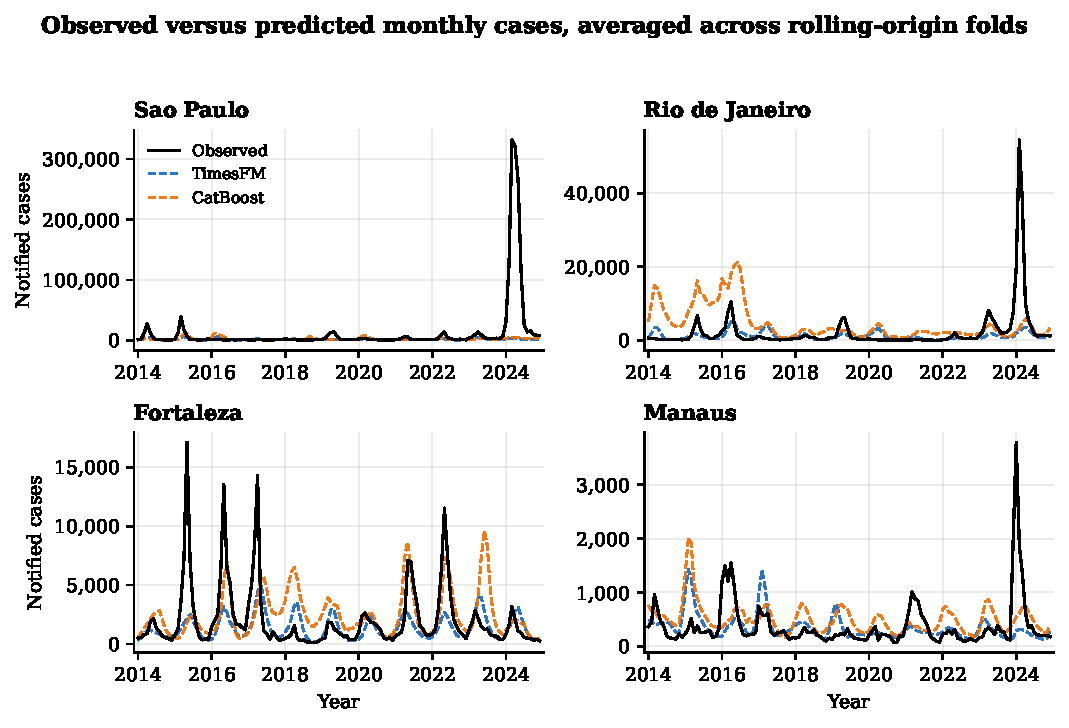
\includegraphics[width=\textwidth]{fig5_observed_vs_predicted.pdf}
\caption{Observed and predicted monthly cases in four cities, with predictions averaged
across all rolling-origin folds covering each month. Both models track the inter-epidemic
baseline and neither reproduces the 2024 peak. CatBoost is shown as the best
purpose-trained model by mean sMAPE.}
\label{fig:obspred}
\end{figure}

% =============================================================================
\section{Prediction interval calibration in full}

Table~\ref{tab:intervals} reports coverage at all three nominal levels, sharpness and the
weighted interval score, for every model under both interval constructions. The main text
reports the 95\% level and the temporal collapse; the full table shows that the ordering
by weighted interval score is not preserved between the two constructions, which is why no
probabilistic ranking of models is claimed.

% gerado por scripts/build_paper_assets.py -- nao editar a mao
\begin{table}[htbp]
\centering
\small
\caption{Calibration and sharpness of conformal prediction intervals, averaged over the
eight cities, under two interval constructions.}
\label{tab:intervals}
\begin{tabular}{lcccrc}
\toprule
 & \multicolumn{3}{c}{Empirical coverage (\%)} & & \\
\cmidrule(lr){2-4}
Model & at 50\% & at 80\% & at 95\% & rWIS & Cities best \\
\midrule
\multicolumn{6}{l}{\textit{Multiplicative intervals (residuals calibrated on the log1p scale)}} \\
\quad CatBoost & 49.4 & 76.9 & 91.3 & 0.69 & 5/8 \\
\quad Random Forest & 48.8 & 78.8 & 92.0 & 0.87 & 1/8 \\
\quad XGBoost & 47.9 & 77.2 & 92.0 & 0.97 & 0/8 \\
\quad TimesFM & 48.5 & 77.3 & 91.7 & 1.46 & 2/8 \\
\quad LightGBM & 45.3 & 73.2 & 89.8 & 27.23 & 0/8 \\
\quad Ridge & 57.0 & 84.2 & 95.9 & 29.44 & 0/8 \\
\quad SARIMAX & 56.2 & 81.2 & 93.9 & 77.77 & 0/8 \\
\addlinespace[4pt]
\multicolumn{6}{l}{\textit{Additive intervals (residuals calibrated on the raw scale)}} \\
\quad TimesFM & 50.9 & 79.2 & 92.0 & 0.59 & 6/8 \\
\quad Ridge & 54.3 & 82.5 & 94.0 & 0.63 & 1/8 \\
\quad CatBoost & 47.9 & 75.7 & 90.3 & 0.68 & 0/8 \\
\quad SARIMAX & 50.7 & 80.1 & 93.7 & 0.70 & 0/8 \\
\quad Random Forest & 48.3 & 77.1 & 91.5 & 0.73 & 1/8 \\
\quad XGBoost & 48.2 & 77.2 & 91.6 & 0.78 & 0/8 \\
\quad LightGBM & 39.2 & 68.5 & 86.1 & 0.81 & 0/8 \\
\bottomrule
\end{tabular}

\vspace{0.5em}
\begin{minipage}{\textwidth}
\footnotesize
Coverage is the percentage of observations falling inside the interval; a value close to
the nominal level indicates calibration. rWIS is the weighted interval score divided by
the city's mean observed count, which makes it comparable across cities; lower is better.
Cities best counts the cities in which a model achieved the lowest rWIS. Intervals are
calibrated only on residuals from earlier folds, so the first 20 folds of each series
carry no interval and 1{,}212 of the 1{,}452 predictions per model per city are
evaluated. The two blocks differ solely in the scale on which residuals are calibrated.
The ordering by rWIS is not preserved between them, and that is why both are reported and
no probabilistic ranking of the models is claimed.
\end{minipage}
\end{table}


\begin{figure}[htbp]
\centering
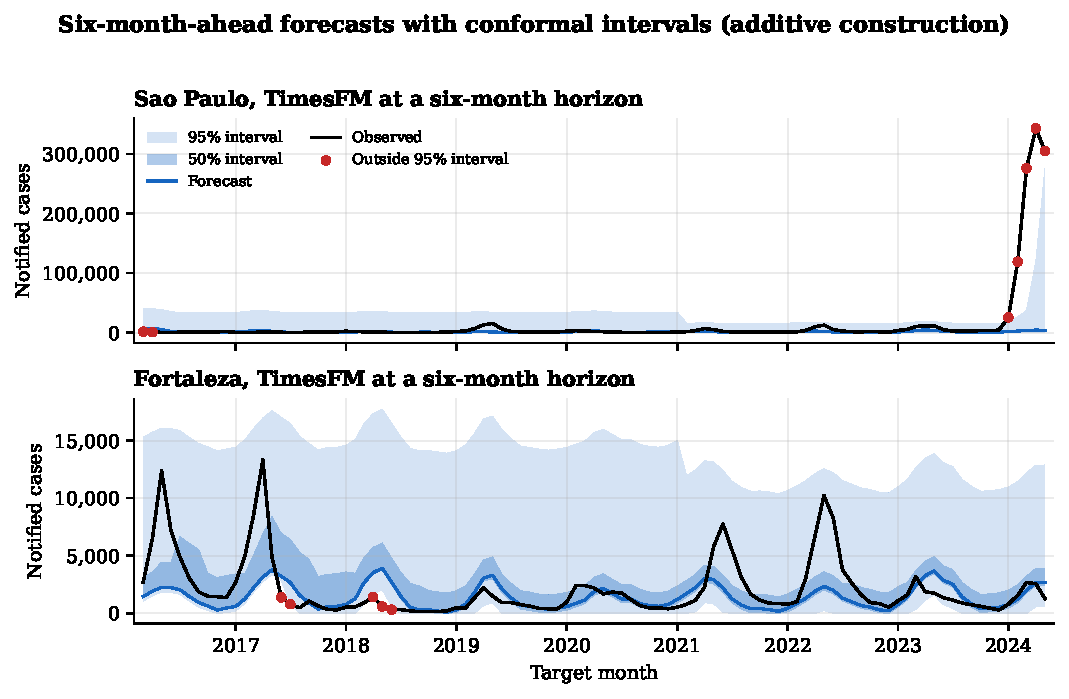
\includegraphics[width=\textwidth]{fig7_fan.pdf}
\caption{Six-month-ahead TimesFM forecasts with additive conformal intervals for two
cities. Red points mark observations falling outside the 95\% interval. S\~ao Paulo shows
the 2024 epidemic breaching the band for several consecutive months. Fortaleza shows the
opposite failure of the additive construction: within a horizon the width is constant, so
the band is far wider than the series through the inter-epidemic period.}
\label{fig:fan}
\end{figure}

% =============================================================================
\section{Model combinations by city}

Figure~\ref{fig:ensembles} gives the per-city outcome summarised in the main text: the
best combination beats the best single model of that city only in S\~ao Paulo, and by a
small margin.

\begin{figure}[htbp]
\centering
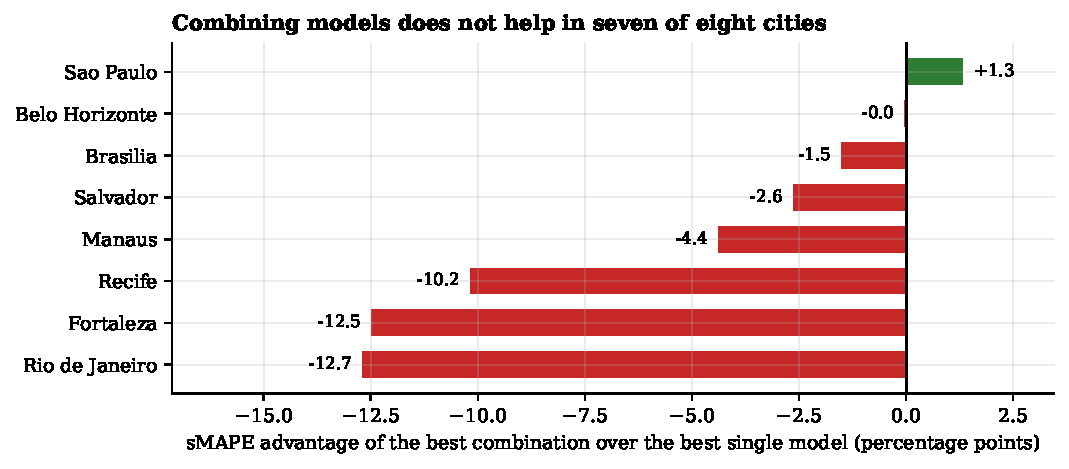
\includegraphics[width=\textwidth]{fig8_ensembles.pdf}
\caption{Difference in sMAPE between the best model combination and the best single model,
by city. Positive values, in green, mean the combination wins. Only S\~ao Paulo favours
combining.}
\label{fig:ensembles}
\end{figure}

\end{document}
